\documentclass{standalone}
\usepackage{times}
\usepackage{pgfplots}
\pgfplotsset{compat=1.15}
\usepackage{mathrsfs}
\usetikzlibrary{arrows,backgrounds,calc,scopes}

%ICPC logo colors
\definecolor{red}{HTML}{972e21}
\definecolor{yellow}{HTML}{ebb83f}
\definecolor{blue}{HTML}{5e7fbf}

\definecolor{green}{HTML}{5fd94e}
\definecolor{cyan}{HTML}{58c9c7}
\definecolor{magenta}{HTML}{d252d3}
\definecolor{lime}{HTML}{96e049}
\definecolor{orange}{HTML}{e78543}
\definecolor{violet}{HTML}{5d5bc4}
\definecolor{purple}{HTML}{9058cb}

\begin{document}
	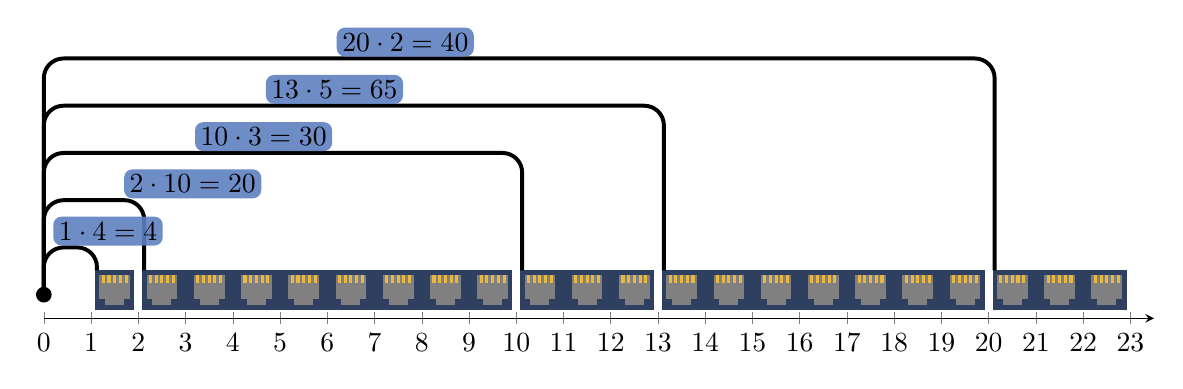
\begin{tikzpicture}[x=0.6cm,y=0.6cm]
		\begin{axis}[
			grid style={opacity=0.25,color=black},
			x=0.6cm,y=0.6cm,
			axis lines=middle,
			axis y line=none,
			xmin=0,
			xmax=23.5,
			ymin=0,
			ymax=1,
			xtick={0.0,...,23.0},]
		\end{axis}
		
		\node[circle,fill,inner sep=2pt] at (0,0.5) {};
		\newcommand{\placeSwitch}[4]{
			%#1 pos,#2 cost, #3 length, #4 line height
			\begin{scope}[on background layer]
				\draw[line width=0.1cm,white,fill=blue!50!black] (#1,0.1) rectangle (#1+#3,1.1);
				\draw[line width=0.05cm,rounded corners=0.25cm] (0,0.5) -- (0,#4+0.5) -| (#1+0.125,1.0165);
			\end{scope}					
			\node[fill=blue,text opacity=1,fill opacity=0.9,rounded corners=3pt,anchor=south west,inner sep=2pt, outer sep=0pt] at (1.5*#4-1.5+0.2,#4+0.54) {
				\pgfmathparse{#1*#2}
				%$#1cm\cdot{}#2\sfrac{\mbox{\footnotesize€}}{cm}=\pgfmathprintnumber{\pgfmathresult}\mbox{€}$
				$#1\cdot{}#2=\pgfmathprintnumber{\pgfmathresult}$
			};					
			\foreach \socket in {1,...,#3} {
				\def\offset{0.175}
				\fill[gray] (\socket+#1-1+\offset,0.23+\offset) rectangle (\socket+#1-\offset,1.1-\offset);
				\def\offset{0.3}
				\fill[gray] (\socket+#1-1+\offset,0.275) rectangle (\socket+#1-\offset,0.6);
				\foreach \pin in {0,...,4} {
					\def\pinLength{0.066}
					\def\pinGap{0.055}
					\def\pinStart{0.225+\pinLength*\pin+\pinGap*\pin}
					\fill[yellow] (\socket+\pinStart+#1-1,0.75) rectangle (\socket+\pinStart+#1-1+\pinLength,0.925);
				}
			}
		}		
		\placeSwitch{1}{4}{1}{1}
		\placeSwitch{2}{10}{8}{2}
		\placeSwitch{10}{3}{3}{3}
		\placeSwitch{13}{5}{7}{4}
		\placeSwitch{20}{2}{3}{5}
	\end{tikzpicture}
\end{document}